
%(BEGIN_QUESTION)
% Copyright 2011, Tony R. Kuphaldt, released under the Creative Commons Attribution License (v 1.0)
% This means you may do almost anything with this work of mine, so long as you give me proper credit

Examine the overhead product pressure control loop (\#33) in this distillation system (in the upper-right corner of the P\&ID).  Suppose PR-33 shows a pressure of 48.1 PSI, while PIC-33 shows a pressure of 50.0 PSI (equal to setpoint):

$$\includegraphics[width=15.5cm]{i0001rx01.eps}$$

Identify which faults could account for the pressure indication discrepancy:

% No blank lines allowed between lines of an \halign structure!
% I use comments (%) instead, so that TeX doesn't choke.

$$\vbox{\offinterlineskip
\halign{\strut
\vrule \quad\hfil # \ \hfil & 
\vrule \quad\hfil # \ \hfil & 
\vrule \quad\hfil # \ \hfil \vrule \cr
\noalign{\hrule}
%
% First row
{\bf Fault} & {\bf Possible} & {\bf Impossible} \cr
%
\noalign{\hrule}
%
% Another row
PR-33 calibration error &  &  \cr
%
\noalign{\hrule}
%
% Another row
PT-33 calibration error &  &  \cr
%
\noalign{\hrule}
%
% Another row
PIC-33 (input) calibration error &  &  \cr
%
\noalign{\hrule}
%
% Another row
PY-33a calibration error &  &  \cr
%
\noalign{\hrule}
%
% Another row
PY-33b calibration error &  &  \cr
%
\noalign{\hrule}
%
% Another row
PV-33a calibration error &  &  \cr
%
\noalign{\hrule}
%
% Another row
PV-33b calibration error &  &  \cr
%
\noalign{\hrule}
} % End of \halign 
}$$ % End of \vbox

\underbar{file i03514}
%(END_QUESTION)





%(BEGIN_ANSWER)

% No blank lines allowed between lines of an \halign structure!
% I use comments (%) instead, so that TeX doesn't choke.

$$\vbox{\offinterlineskip
\halign{\strut
\vrule \quad\hfil # \ \hfil & 
\vrule \quad\hfil # \ \hfil & 
\vrule \quad\hfil # \ \hfil \vrule \cr
\noalign{\hrule}
%
% First row
{\bf Fault} & {\bf Possible} & {\bf Impossible} \cr
%
\noalign{\hrule}
%
% Another row
PR-33 calibration error & $\surd$ &  \cr
%
\noalign{\hrule}
%
% Another row
PT-33 calibration error &  &  $\surd$ \cr
%
\noalign{\hrule}
%
% Another row
PIC-33 (input) calibration error & $\surd$ &  \cr
%
\noalign{\hrule}
%
% Another row
PY-33a calibration error & $\surd$ &  \cr
%
\noalign{\hrule}
%
% Another row
PY-33b calibration error &  & $\surd$ \cr
%
\noalign{\hrule}
%
% Another row
PV-33a calibration error &  & $\surd$ \cr
%
\noalign{\hrule}
%
% Another row
PV-33b calibration error &  & $\surd$ \cr
%
\noalign{\hrule}
} % End of \halign 
}$$ % End of \vbox


%(END_ANSWER)





%(BEGIN_NOTES)


\filbreak \vskip 20pt \vbox{\hrule \hbox{\strut \vrule{} {\bf Virtual Troubleshooting} \vrule} \hrule}

\noindent
{\bf Predicting the effect of a given fault:} present each of the following faults to the students, one at a time, having them comment on all the effects each fault would produce.

\begin{itemize}
\item{} 
\item{} 
\item{} 
\end{itemize}


\vskip 10pt


\noindent
{\bf Identifying possible/impossible faults:} present symptoms to the students and then have them determine whether or not a series of suggested faults could account for all the symptoms, explaining {\it why} or {\it why not} for each proposed fault:

\begin{itemize}
\item{} Symptom: {\it Liquid level in vessel V-13 above setpoint and trending upward}
\item{} IAS supply failure to FV-31 -- {\bf No}
\item{} LIC-30 in manual mode -- {\bf Yes}
\item{} FF segment LAS failed, with no backup -- {\bf No}
\item{} FC-31 in manual mode -- {\bf Yes}
\item{} Missing terminator on FF segment -- {\bf No}
\item{} Device hosting FC-31 failed -- {\bf Yes}
\item{} Too little unscheduled time on FF segment -- {\bf No}
\item{} FT-31 zero shift (reading 5\% too high) -- {\bf No}
\item{} FT-31 zero shift (reading 5\% too low) -- {\bf No}
\end{itemize}


\vskip 10pt


\noindent
{\bf Determining the utility of given diagnostic tests:} present symptoms to the students and then propose the following diagnostic tests one by one.  Students rate the value of each test, determining whether or not it would give useful information (i.e. tell us something we don't already know).  Students determine what different results for each test would indicate about the fault, if anything:

\begin{itemize}
\item{} Symptom: {\it FV-31 remains at a fixed position no matter the output value of FC-31, but FT-31's reading is still showing true on the DCS display}
\item{} Measure FF segment signal using an oscilloscope -- {\bf No}
\item{} Place the PID function block in manual mode and change its output value -- {\bf No}
\item{} Place the AO function block in manual mode and change its output value -- {\bf Yes}
\item{} Measure FF segment DC voltage using a multimeter -- {\bf No}
\item{} Check the status of the segment's LAS -- {\bf No}
\item{} Examine a ``live'' display of all variables between function blocks -- {\bf Yes}
\item{} Check for at least 70\% unscheduled (acyclic) time on the FF segment -- {\bf No}
\end{itemize}


\vskip 10pt


\noindent
{\bf Diagnosing a fault based on given symptoms:} imagine the ??? fails ??? in this system (don't reveal the fault to students!).  Present the operator's observation(s) to the students, have them consider possible faults and diagnostic strategies, and then tell them the results of tests they propose based on the following symptoms, until they have properly identified the nature and location of the fault:

\begin{itemize}
\item{} Operator observation: {\it }
\item{} 
\item{} 
\end{itemize}
%INDEX% Basics, control loop troubleshooting (realistic P&ID shown)
%INDEX% Measurement, pressure: troubleshooting
%INDEX% Process: distillation, generic (realistic P&ID shown)

%(END_NOTES)

